\section{Contextualization}

URDAD, the {\em Use-Case, Responsibility-Driven Analysis and Design} \cite{solms_urdad_2010, solms_generating_2009, solms_technology_2007} method, is a method used by requirements specialists (typically business analysts) to perform technology neutral, services oriented analysis and business process design. The resultant analysis and business process design models are meant to be augmented by technical experts to formalize conditions and constraints.

The output of the URDAD method is an URDAD model containing the requirements and technology neutral process design. Historically the URDAD model has been encoded in UML. Such an encoding suffers from impresice semantics, excessive model complexity and high model defect rates caused by the size and complexity of UML and the high level of discipline required to encode an URDAD model in UML.

To address these issues and metamodel introducing only the URDAD model features has been developed. This metamodel forms the basis for a {\em Domain-Specific Language} (DSL) for URDAD.  The model is meant to be populated through the use of concrete text and diagrammatic syntaxes defined for the URDAD DSL. Currently a concrete EMFText-based syntax is available.

An URDAD model recursively assembles higher level services from lower level services. The leaf services are services sourced from the environment. These include services provided by the implementation language/technologies, persistence services and services sourced from external systems. For each service the the URDAD model contains
\begin{itemize}
 \item the \textit{service contract} with data structure specification for the request (input) and result (output) object as well as pre- and post-conditions used for functional testing and quality requirements used for testing non-functional requirements,
 \item the \textit{service} specification specifying the functional requirements (i.e.\ lower level services from which this higher level service is assembled), and the actual orchestration of the process for the service across these lower level services. The outcome of the service is either the result object (return value) or the notification that the service is not provided due to a particular pre-condition not having been met by raising the exception for that pre-condition.
\end{itemize}

\subsection{The URDAD meta-model}

The URDAD metamodel specifies the model structure for the input model of the transformation. It is encoded in Ecore and is encluded in the artifacts provided to the mapping teams. Figure \ref{fig:metamodel} shows a diagrammatic representation of the metamodel. 

\begin{figure}
  \centering
  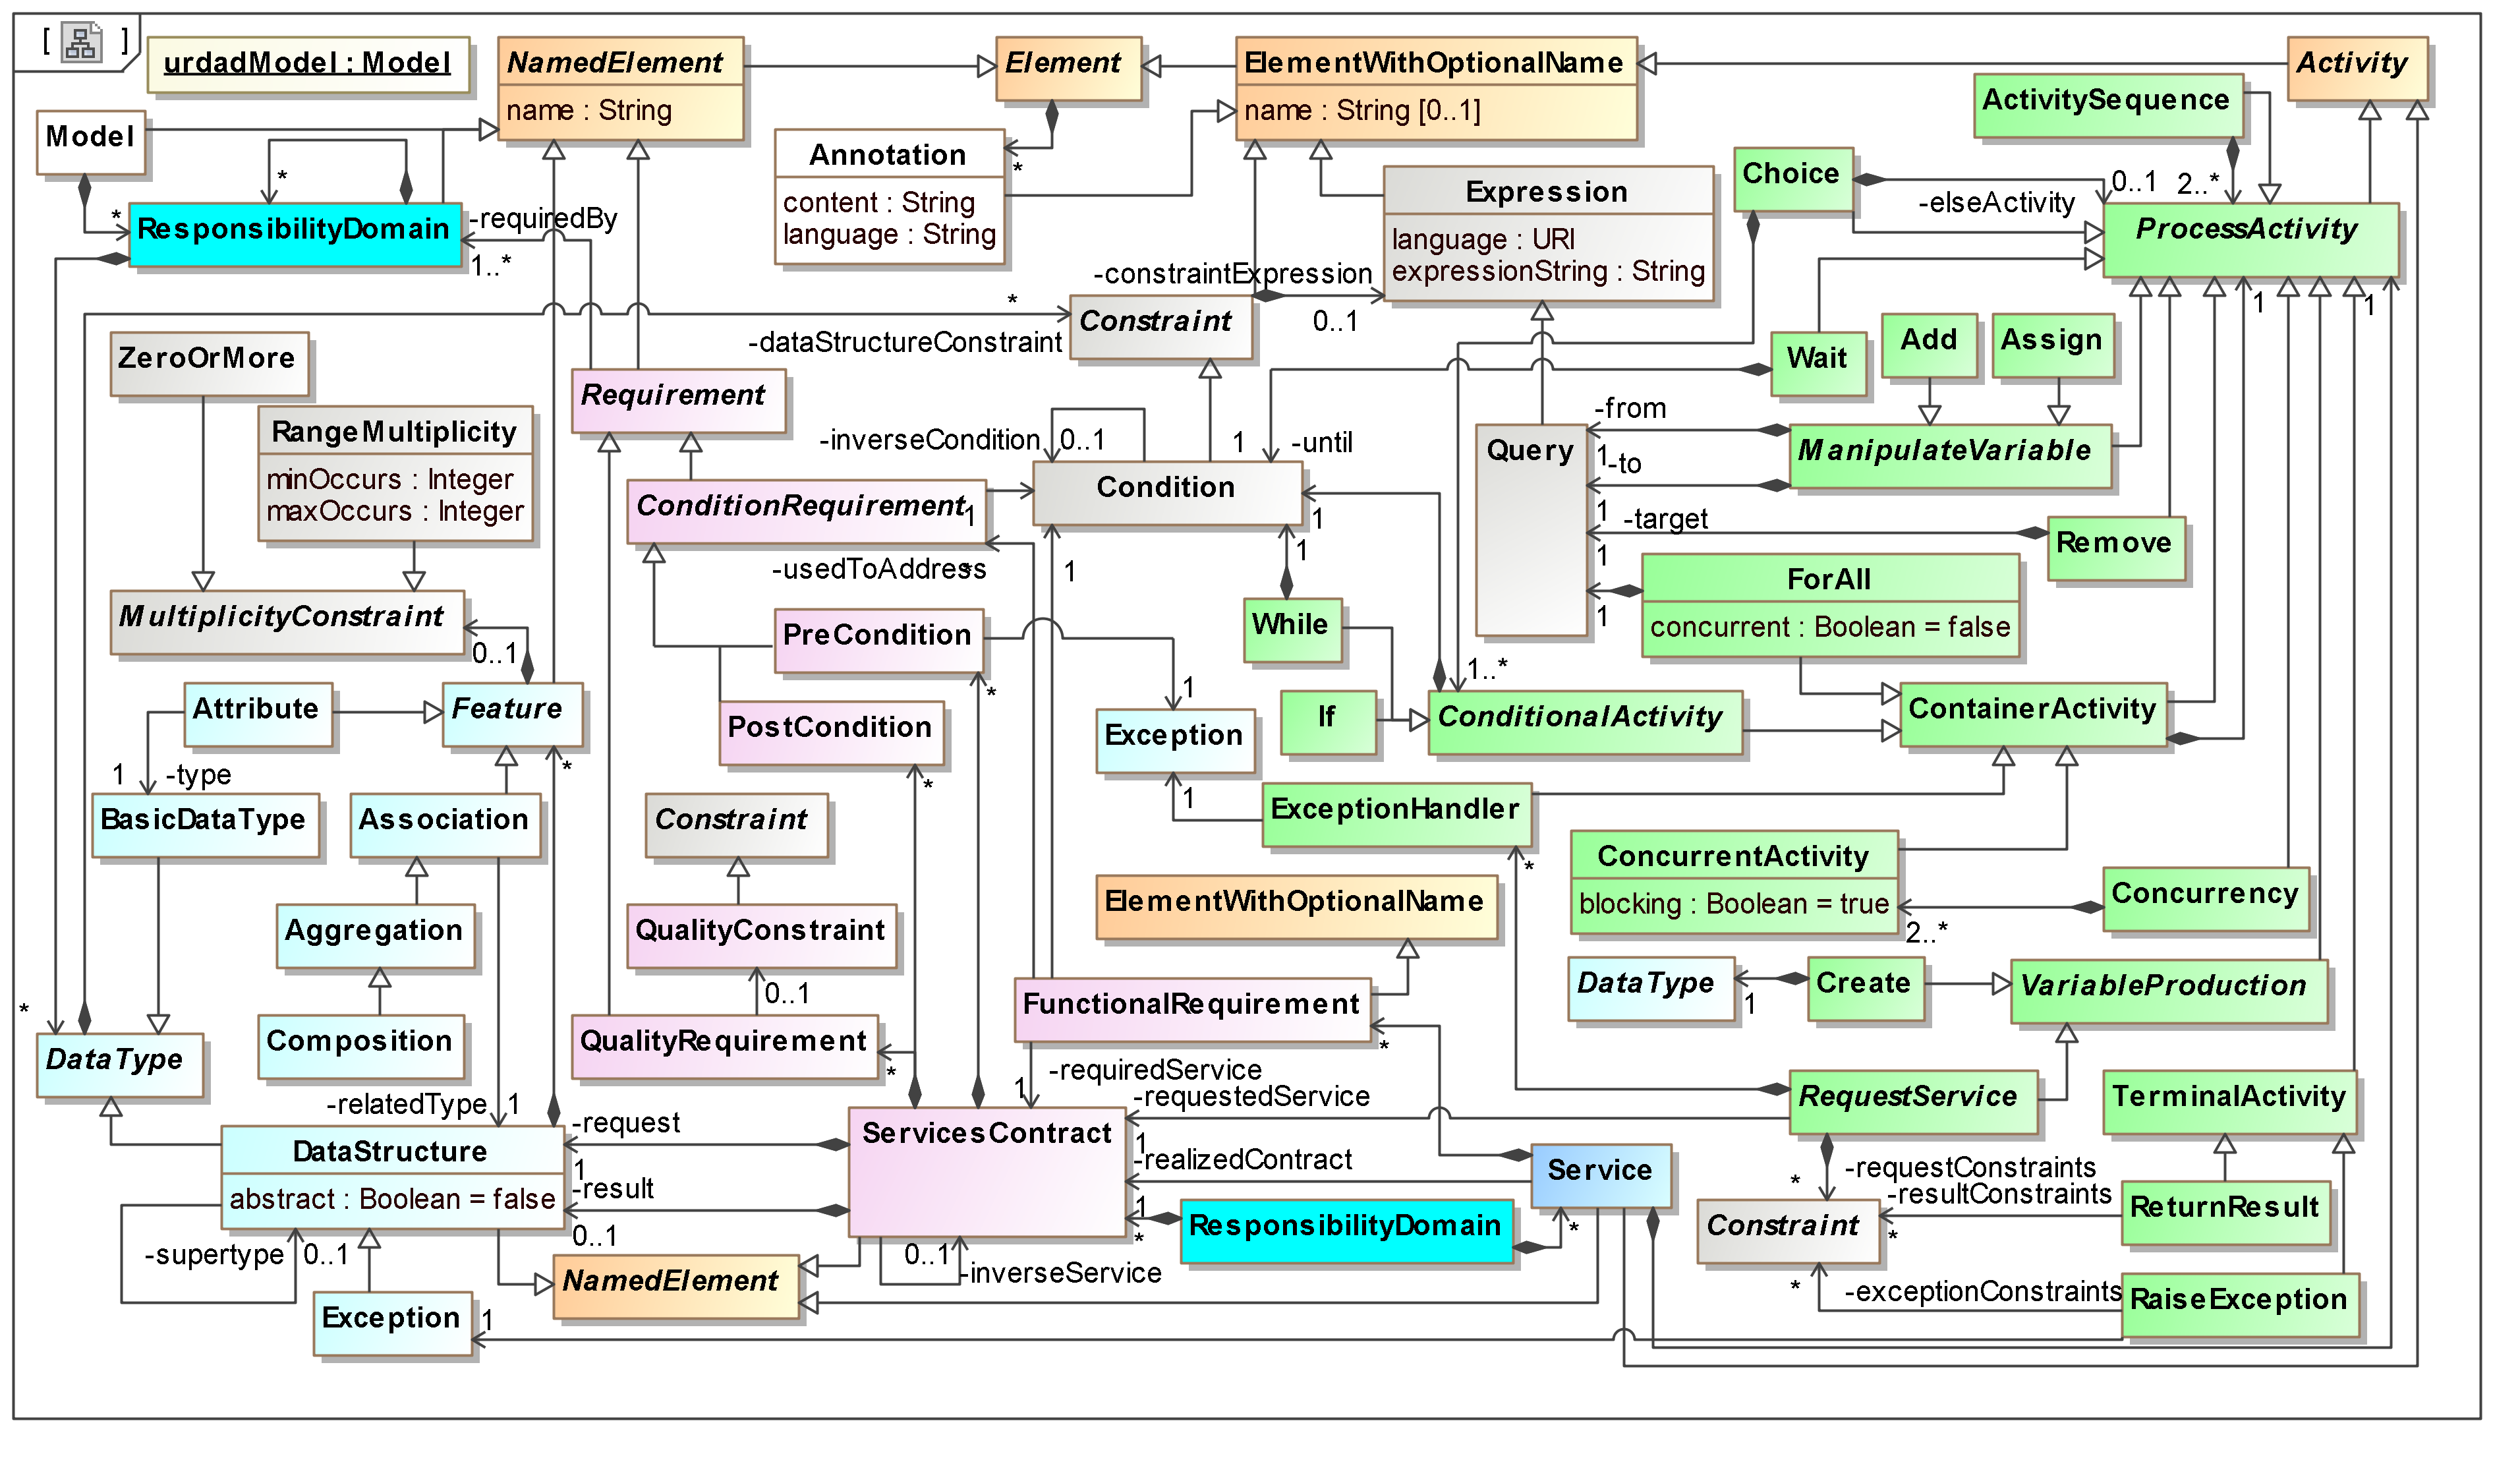
\includegraphics{metamodel}
  \caption{A diagrammatic representation of the URDAD metamodel}
  \label{fig:metamodel}
\end{figure}


